\section{System}
\label{sec:system}

\subsection{Architecture}

DMCP Studio is a static single-page front-end over a FastAPI back-end whose job
is to wrap the published DynamicMCPBench pipeline and the Benchmark Advisor
services through thin adapters. The end-to-end flow is: user intent
$\rightarrow$ Advisor statistical plan $\rightarrow$ guarded corpus generation
$\rightarrow$ collect/explore/distill/score. The adapter exposes one function
per pipeline stage and returns the pipeline's own \texttt{pydantic} models; the
back-end never reimplements distillation or scoring, and the Advisor stays
side-effect-free until the user confirms a guarded corpus-only handoff. The two
slow stages---exploration and candidate scoring---stream call-by-call over
Server-Sent Events (SSE), so the UI fills as the agent acts. This ``wrap, don't
rewrite'' boundary is what lets us claim the studio shows the real system: every
verdict on screen is computed by the same code path the methodology paper
reports, and every launchable design uses the same contract the generation
pipeline consumes.

\subsection{Stage 0: designing the benchmark}
\label{sec:advisor}

Benchmark Advisor is a pre-generation statistical design assistant
(Figure~\ref{fig:advisor}): it decides what a planned benchmark can support
before the user spends time generating a corpus. From a natural-language
evaluation question plus optional structure (comparison mode, candidate models,
task budget, attempts, requested detectable effect, server scope, and task mix)
it returns a \texttt{StatisticalPlan}: a scoped claim, method choice, assumption
ledger, power curve, issues and repairs, alternatives, and guide citations.

\begin{figure}[tbp]
  \centering
  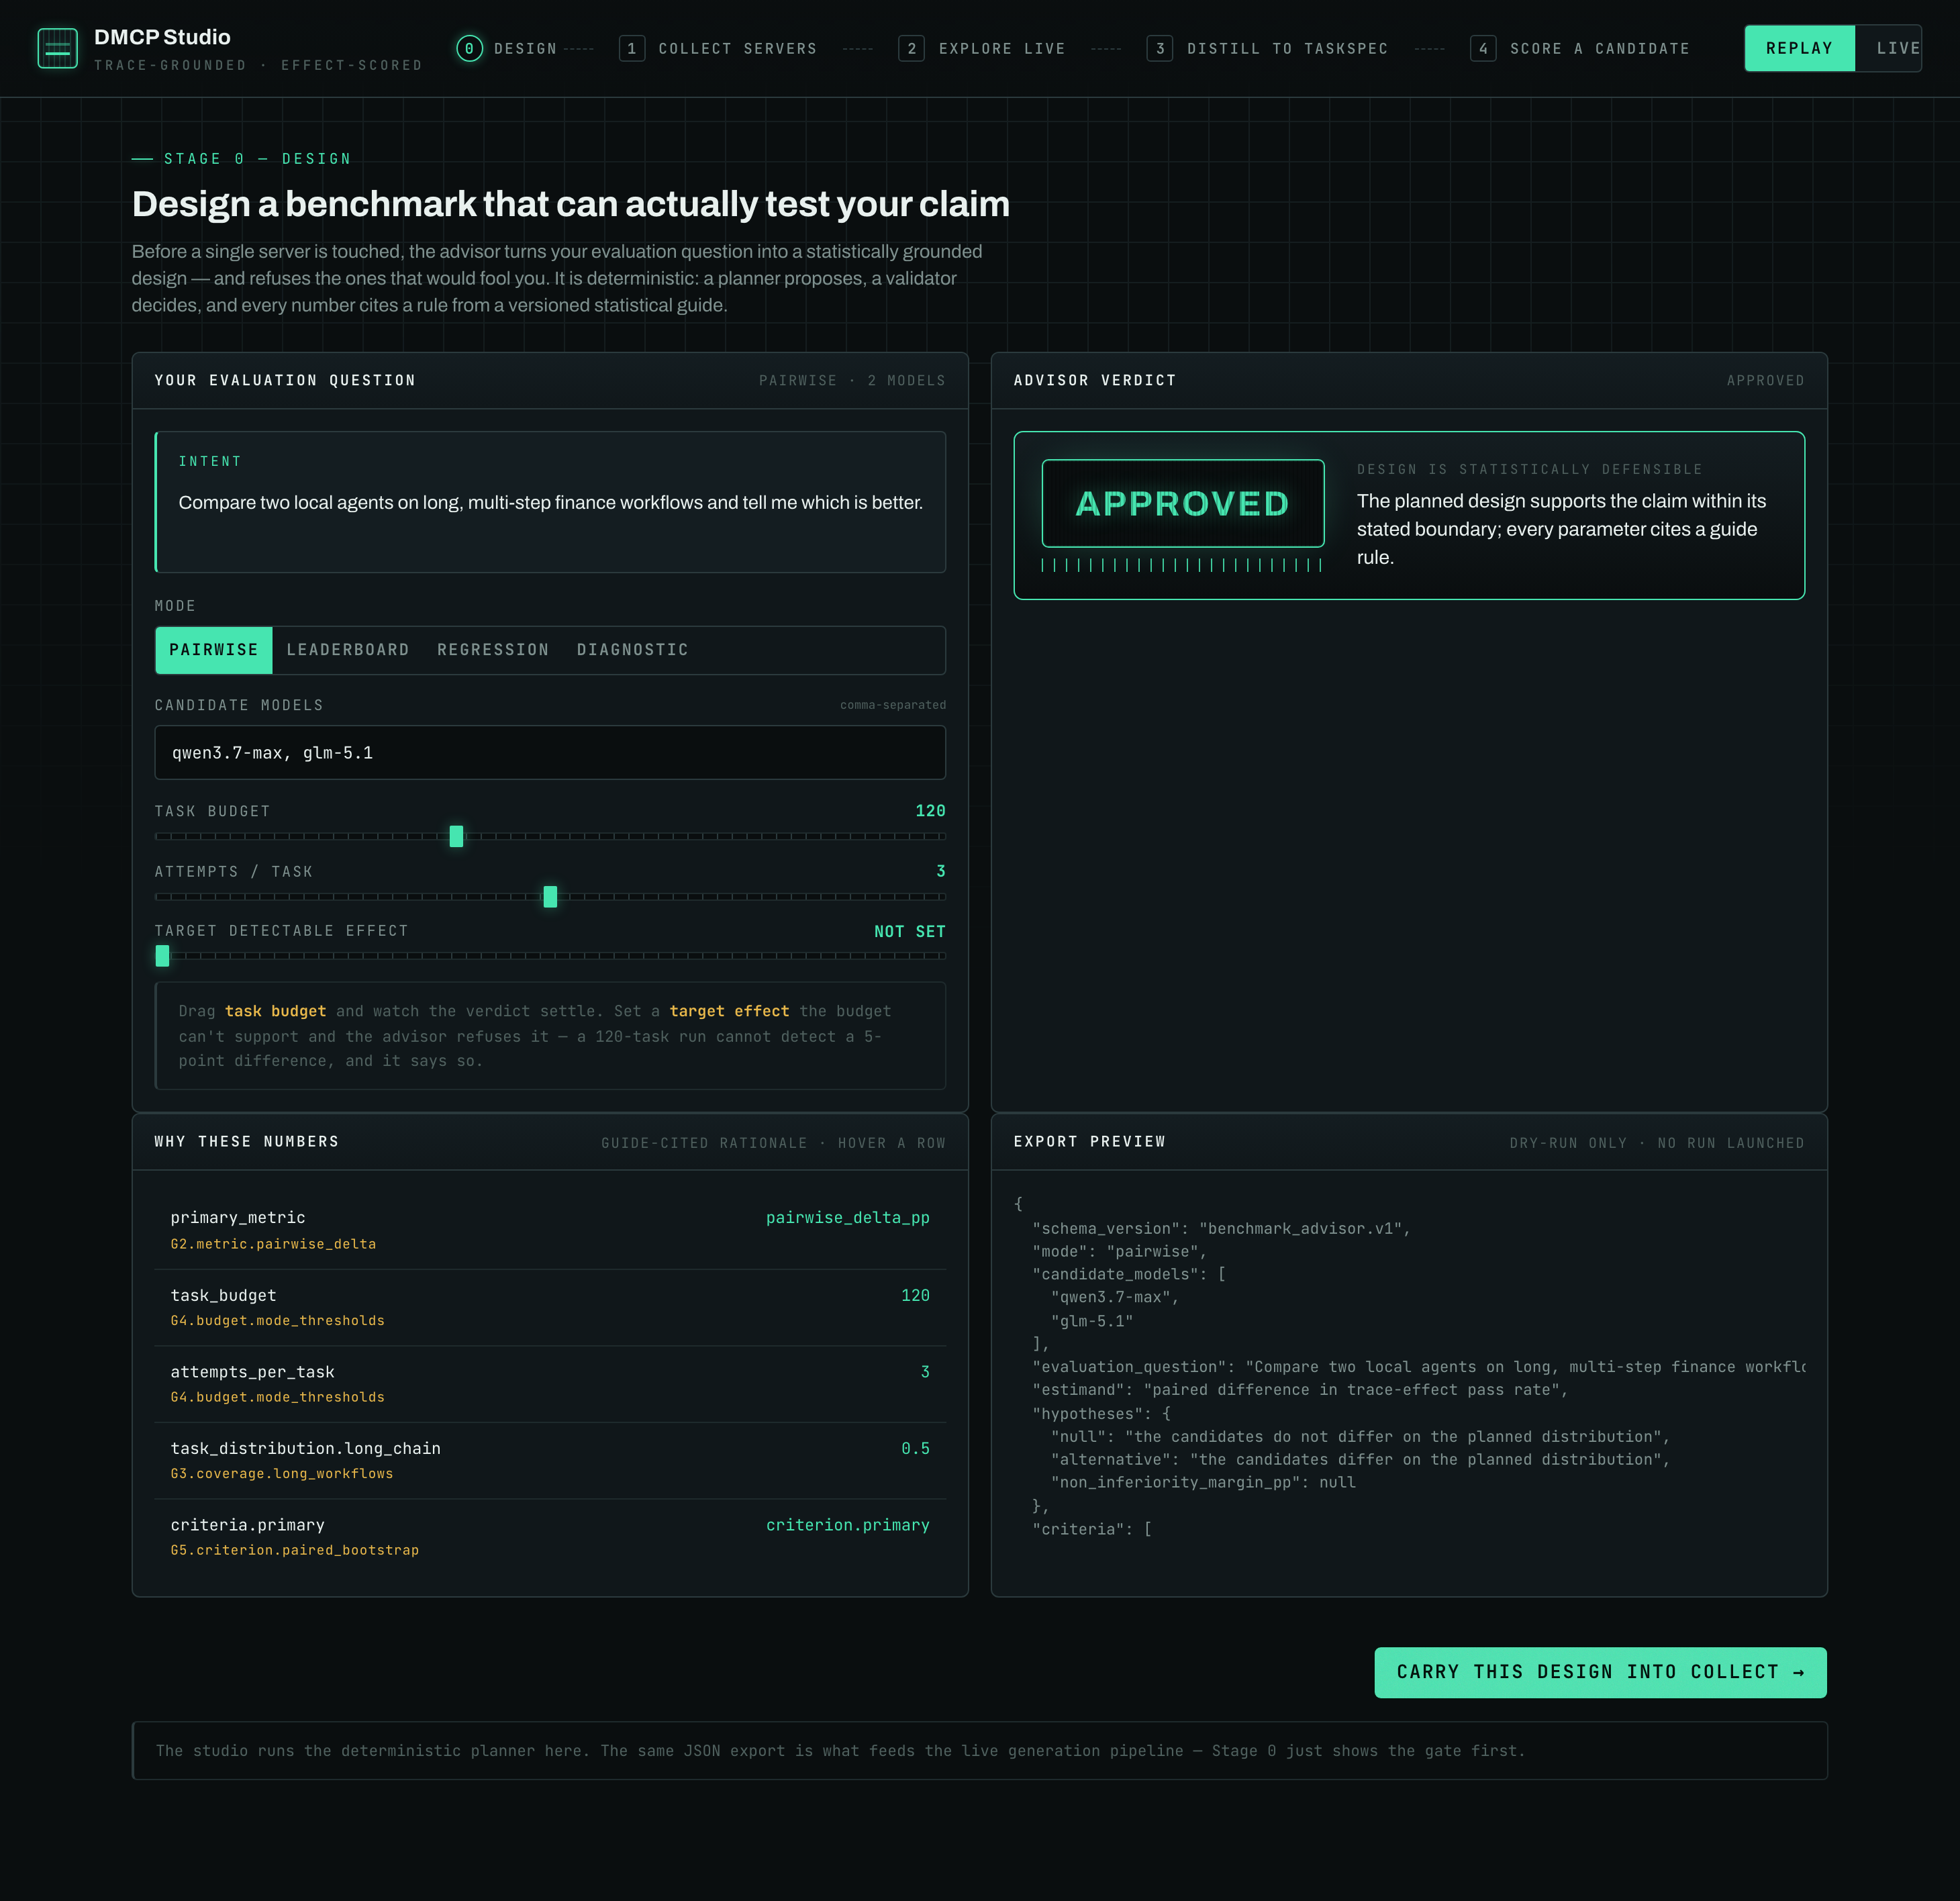
\includegraphics[width=\columnwidth]{figures/fig_advisor.png}
  \caption{\textbf{Stage 0 --- Design.} Benchmark Advisor turns an evaluation
    question into a statistically scoped benchmark plan before generation. The
    workbench shows the supported claim, MDE and power diagnostics, assumptions,
    repair actions, alternatives, and guide citations. Approved or warning-level
    plans can be carried forward only through an explicit guarded handoff to
    corpus/specs/traces generation. A full-width version appears in
    Figure~\ref{fig:advisor-full}.}
  \label{fig:advisor}
\end{figure}

The design loop is guide-first and deterministic. A curated
\texttt{STATISTICAL\_GUIDE.md} maps intent signals to mode, metric, budget and
repeat policy, criterion, and claim boundary; the engine then searches a finite
grid of candidate budgets, attempt counts, and effect targets, validates each
with deterministic rules, and labels it \textsf{approved}, \textsf{warning}, or
\textsf{refused}. The recommendation is not a UI default but the cheapest
sufficient candidate, with stronger and narrowed-claim alternatives kept
visible. Its core diagnostic is the pre-run minimum detectable effect: for a
binary effect-pass metric the Advisor uses
$\mathrm{MDE} \approx (z_{1-\alpha/2} + z_{1-\beta})\sqrt{2p(1-p)/n_{\mathrm{eff}}}$
(no-prior defaults $p=0.5$, $\alpha=0.05$, power $0.80$). Crucially
$n_{\mathrm{eff}} \leq$ the number of \emph{unique} tasks: repeated attempts
support reliability analysis but do not multiply the independent sample size, so
a 40-task smoke run and a 500-task selection run make visibly different claims
before either is launched.

Launchability is separate from approval text. Refused or under-specified designs
export nothing; approved or warning-level designs carry into Collect only through
an explicit confirmation restricted to corpus/specs/traces generation. The
Advisor never starts leaderboard evaluation or paid scoring---it gates and
documents the benchmark the rest of the system will generate.

\subsection{Four stages}

\paragraph{1. Collect.} The visitor points the studio at MCP servers---the
three public servers from the worked example, or any server URL---and the
collector returns each server's tool surface tagged by dynamism (live-read
vs.\ stateful-write). State-changing servers are marked and, per the sandbox
rule (Ethical Considerations), never invoked unless flagged sandboxed. If an
Advisor plan was carried forward, Collect uses its task budget, server scope,
and task-distribution constraints as the generation contract.

\paragraph{2. Explore.} A goal generator turns the selected tool surface into a
realistic user request; an explorer agent then pursues it \emph{live}, and every
successful tool call streams into a reference trace. Generation is forward: we
explore first and distill second, so no tool dependency graph is ever imposed.
Tool names are visible to the explorer here but stripped from the candidate's
prompt later, so a candidate cannot copy the reference path.

\paragraph{3. Distill.} Unlike a fixed tool-list grader, a checkpoint is not a
required reference call: it is an observable effect with admissible
realizations, argument constraints, and, when needed, value-level evidence. The
distiller compiles the recorded trace into a path-agnostic \emph{TaskSpec}: a
set of effect checkpoints (a tool effect, demanding that \emph{some} tool from
an equivalence set ran with the right arguments, or a \emph{value-produced}
effect), optional forbidden-action minefields, and a partial order. Because
every checkpoint comes from a tool that was actually used to reach the goal, a
spurious ``unnecessary tool'' cannot appear. The studio renders each checkpoint
as a card and---crucially---renders equivalence sets as \textbf{editable chips}
the visitor can toggle.

\paragraph{4. Score.} The visitor picks a candidate agent and watches its
trajectory replay against the checkpoint ledger. The scoring endpoint returns
\emph{both} an effect verdict and an answer verdict on every call; the
Effect/Answer toggle is therefore a pure front-end re-render over one payload,
never a second backend call. We define \texttt{answer\_pass} as a demo-only
answer-matching baseline: the candidate's final message is compared with the
recorded reference final answer after simple normalization; it is independent of
the trace and is never used as the DynamicMCPBench verdict. Toggling an
equivalence-set member re-scores Tier-1 effects live, so the visitor can watch a
pass become a failure by disabling the very tool the candidate happened to use.

\subsection{The verdict flip}

The studio is organized around making answer-matching and effect-scoring
\emph{disagree on screen}. Three curated cases (frozen as REPLAY fixtures,
\S\ref{sec:eval}) each reproduce a different disagreement:

\begin{enumerate}\itemsep2pt
  \item \textbf{Equivalent-tool pass.} The candidate reaches the price-history
    effect with \texttt{get\_price\_history} where the reference used
    \texttt{download}. Effect-scoring passes it via the equivalence set; a
    tool-list grader would flag a ``wrong'' tool.
  \item \textbf{Answer-pass, effect-fail.} A fluent agent skips the
    income-statement step, then writes a confident summary. Answer-matching
    accepts the prose; effect-scoring marks the missing checkpoint
    \textsf{unmet}. This \emph{incomplete-aggregation} failure is the dominant
    failure mode in the parent study.
  \item \textbf{Answer-fail, effect-pass.} A correct agent reports live returns
    that no longer match the stored reference string. Answer-matching penalizes
    a genuinely correct run; effect-scoring passes it. This is exactly the
    fragility of grading the answer on live data.
\end{enumerate}

\subsection{LIVE vs.\ REPLAY}

A mode switch in the header backs every stage with either real pipeline calls
(LIVE) or frozen fixtures served deterministically (REPLAY). REPLAY is the
public default: it makes the demo reproducible on a booth laptop and is
on-thesis, because the methodology grades under deterministic replay. LIVE
drives the real pipeline against read-only servers as proof, with per-stage
timeouts and a graceful fall-back to the REPLAY fixture if a live server is
unreachable, so a flaky network never bricks the demo. The headline verdict uses
Tier-1 deterministic scoring (matching the paper); the optional Tier-2
effect-equivalence judge is shown as an upgrade, never on the critical path.
